% !TEX program = pdflatex
% !TEX TS-program = pdflatex
\documentclass[11pt,a4paper]{article}

% ---------------------------------------------------------------------------
% Encoding, language and typography
% ---------------------------------------------------------------------------
\usepackage[T1]{fontenc}        % proper 8-bit font encoding
\usepackage{lmodern}            % scalable Latin Modern fonts
\usepackage[english]{babel}     % language rules (hyphenation, also used by spell checkers)
\usepackage{csquotes}           % correct quotation marks: \enquote{...}
\usepackage{microtype}          % better justification and spacing
\usepackage{setspace}           % line spacing control
\setstretch{1.0}

% ---------------------------------------------------------------------------
% Page layout and headers
% ---------------------------------------------------------------------------
\usepackage[a4paper,margin=2.0cm]{geometry}
\usepackage{fancyhdr}
\usepackage{lastpage}
\pagestyle{fancy}
\fancyhf{}
\fancyhead[L]{COMP4212 --- Backpropagation in one example}
\fancyfoot[C]{\thepage\ of \pageref{LastPage}}
\renewcommand{\headrulewidth}{0.4pt}
\setlength{\headheight}{14pt}

% ---------------------------------------------------------------------------
% Mathematics
% ---------------------------------------------------------------------------
\usepackage{amsmath}            % core math environments
\usepackage{amssymb}            % extra symbols (\mathbb, \nexists, ...)
\usepackage{amsfonts}
\usepackage{mathtools}          % fixes and extensions to amsmath
\usepackage{bm}                 % bold math symbols: \bm{\beta}
\usepackage{dsfont}             % indicator function \mathds{1}

\DeclareMathOperator{\argmin}{arg\,min}
\DeclareMathOperator{\argmax}{arg\,max}
\DeclareMathOperator{\relu}{ReLU}

\newcommand{\pd}[2]{\frac{\partial #1}{\partial #2}}
\newcommand{\code}[1]{\texttt{#1}}

% ---------------------------------------------------------------------------
% Figures, tables, lists
% ---------------------------------------------------------------------------
\usepackage{graphicx}
\usepackage{booktabs}           % professional tables
\usepackage{enumitem}           % customizable lists
\usepackage{xcolor}
\usepackage{tikz}
\usetikzlibrary{positioning,arrows.meta}
\usepackage[most]{tcolorbox}

\newtcolorbox{keybox}[1]{colback=blue!4,colframe=blue!50!black,fonttitle=\bfseries,title={#1}}

\colorlet{fwd}{blue!70!black}
\colorlet{bwd}{red!75!black}

% ---------------------------------------------------------------------------
% Hyperlinks and cross-references (load last)
% ---------------------------------------------------------------------------
\usepackage[hidelinks]{hyperref}
\usepackage[capitalise,noabbrev]{cleveref}

\hypersetup{
  pdftitle={Backpropagation in One Example},
  pdfsubject={COMP4212 Reinforcement Learning}
}

% ===========================================================================
\begin{document}

\begin{center}
  {\LARGE\bfseries Backpropagation in One Example}\\[0.3em]
  {\large What \code{loss.backward()} actually does}
\end{center}

\section{The problem backpropagation solves}

Training a network means changing every weight $w$ a little in the direction that makes the loss $L$ smaller:
\[
  w \;\gets\; w - \alpha\,\pd{L}{w}\qquad(\alpha=\text{learning rate}).
\]
So for \emph{every} weight we need $\pd{L}{w}$: \enquote{if I increase this weight a tiny bit, how much does the loss change?}
Nudging each of the millions of weights separately and rerunning the network would be far too slow.
\textbf{Backpropagation} gets \emph{all} these derivatives with one forward and one backward pass. It is just the chain rule, applied cleverly.

\section{The only rule you need: the chain rule}

If $L$ depends on $w$ only through an intermediate value $y$, then $\displaystyle\pd{L}{w} = \pd{L}{y}\cdot\pd{y}{w}$.
Rates of change multiply: if $y$ changes 3 times as fast as $w$, and $L$ 4 times as fast as $y$, then $L$ changes $3\cdot4=12$ times as fast as $w$.
A network is a long chain of simple steps, so the derivative w.r.t.\ an early weight is a product of many simple \emph{local} derivatives. Backpropagation computes this product \emph{from the end backwards}, reusing partial products on the way.

\section{Worked example}

\paragraph{The network.} One input $x$, two weights $w_1,w_2$, one ReLU in between, and a squared-error loss against a target $t$:
\[
  z = w_1 x,\qquad h = \relu(z)=\max(0,z),\qquad y = w_2 h,\qquad L = (y-t)^2 .
\]
Numbers: $x=2$, $t=1$ (what we want the network to output), $w_1=0.5$, $w_2=3$.

\begin{figure}[h]
\centering
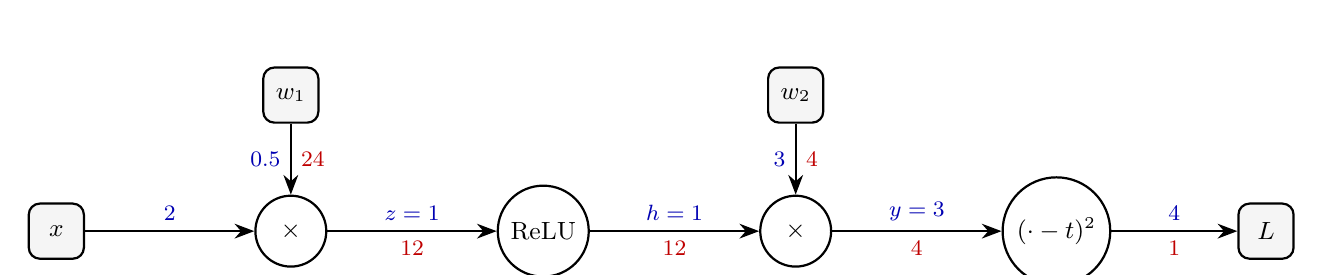
\begin{tikzpicture}[
  node distance=2.15cm,
  op/.style={circle,draw,thick,minimum size=9mm,font=\small},
  inp/.style={rectangle,draw,rounded corners,thick,minimum size=7mm,font=\small,fill=gray!8},
  >={Stealth[length=2.5mm]}]
  \node[inp] (x) {$x$};
  \node[op, right=of x] (m1) {$\times$};
  \node[inp, above=0.9cm of m1] (w1) {$w_1$};
  \node[op, right=of m1] (r) {ReLU};
  \node[op, right=of r] (m2) {$\times$};
  \node[inp, above=0.9cm of m2] (w2) {$w_2$};
  \node[op, right=of m2] (sq) {$(\cdot-t)^2$};
  \node[inp, right=1.6cm of sq] (L) {$L$};

  \draw[->,thick] (x) -- node[above,fwd,font=\footnotesize]{$2$} (m1);
  \draw[->,thick] (w1) -- node[left,fwd,font=\footnotesize]{$0.5$} node[right,bwd,font=\footnotesize]{$24$} (m1);
  \draw[->,thick] (m1) -- node[above,fwd,font=\footnotesize]{$z=1$} node[below,bwd,font=\footnotesize]{$12$} (r);
  \draw[->,thick] (r) -- node[above,fwd,font=\footnotesize]{$h=1$} node[below,bwd,font=\footnotesize]{$12$} (m2);
  \draw[->,thick] (w2) -- node[left,fwd,font=\footnotesize]{$3$} node[right,bwd,font=\footnotesize]{$4$} (m2);
  \draw[->,thick] (m2) -- node[above,fwd,font=\footnotesize]{$y=3$} node[below,bwd,font=\footnotesize]{$4$} (sq);
  \draw[->,thick] (sq) -- node[above,fwd,font=\footnotesize]{$4$} node[below,bwd,font=\footnotesize]{$1$} (L);
\end{tikzpicture}
\caption{The computational graph. \textcolor{fwd}{Blue}: values computed in the forward pass (left to right). \textcolor{bwd}{Red}: the gradient $\partial L/\partial(\cdot)$ of each value, computed in the backward pass (right to left).}
\label{fig:graph}
\end{figure}

\paragraph{Step 1: forward pass (left to right).} Compute and \emph{remember} every intermediate value:
\[
  z = 0.5\cdot2 = 1,\qquad h=\max(0,1)=1,\qquad y=3\cdot1=3,\qquad L=(3-1)^2=4 .
\]
The output is 3 but should be 1, so the loss is 4.

\paragraph{Step 2: backward pass (right to left).} Start at the end with $\pd{L}{L}=1$. At each node, multiply the gradient arriving from the right (\enquote{upstream gradient}) by the node's \emph{local} derivative, which only needs the values remembered from the forward pass:
\begin{center}
\renewcommand{\arraystretch}{1.15}
\begin{tabular}{@{}l l l l@{}}
\toprule
Quantity & Local derivative & Chain rule & Value \\
\midrule
$\partial L/\partial y$ & $\partial (y-t)^2/\partial y = 2(y-t)$ & $1\cdot 2(3-1)$ & $\mathbf{4}$ \\
$\partial L/\partial w_2$ & $\partial y/\partial w_2=h$ & $(\partial L/\partial y)\cdot h = 4\cdot1$ & $\mathbf{4}$ \\
$\partial L/\partial h$ & $\partial y/\partial h=w_2$ & $(\partial L/\partial y)\cdot w_2 = 4\cdot3$ & $\mathbf{12}$ \\
$\partial L/\partial z$ & $\partial h/\partial z=1$ if $z>0$, else $0$ & $(\partial L/\partial h)\cdot1 = 12\cdot1$ & $\mathbf{12}$ \\
$\partial L/\partial w_1$ & $\partial z/\partial w_1=x$ & $(\partial L/\partial z)\cdot x = 12\cdot2$ & $\mathbf{24}$ \\
\bottomrule
\end{tabular}
\end{center}
Notice how $\partial L/\partial w_1$ reused $\partial L/\partial z$, which reused $\partial L/\partial h$, which reused $\partial L/\partial y$. Nothing is computed twice. That reuse is the whole trick, and it is why one backward pass costs about as much as one forward pass, no matter how many weights there are.

\paragraph{Step 3: update the weights.} With learning rate $\alpha=0.01$:
\[
  w_1 \gets 0.5 - 0.01\cdot24 = 0.26,\qquad w_2 \gets 3 - 0.01\cdot4 = 2.96 .
\]

\paragraph{Step 4: check.} New forward pass: $z=0.52$, $h=0.52$, $y=2.96\cdot0.52\approx1.54$, $L=(1.54-1)^2\approx\mathbf{0.29}$.
The loss dropped from 4 to 0.29 in one step. Each gradient told its weight which way to move (both positive, so both weights went down) and how strongly ($w_1$ had the larger gradient, so it moved more).

\paragraph{What if $z$ had been negative?} Then ReLU outputs 0 and its local derivative is 0, so $\pd{L}{z}=0$ and $\pd{L}{w_1}=0$: the gradient is \enquote{blocked} and $w_1$ does not learn from this example. This is how a non-linearity shapes which weights get updated.

\section{The general recipe}

\begin{keybox}{Backpropagation}
\begin{enumerate}[nosep,leftmargin=*]
  \item \textbf{Forward:} compute the output and the loss, storing every intermediate value (this is the \emph{computational graph}).
  \item \textbf{Backward:} start with $\pd{L}{L}=1$ and visit the nodes in reverse order. Each node multiplies the incoming gradient by its local derivative and sends the result to its inputs.
  \item \textbf{If a value feeds into several places}, the gradients coming back from those places are \emph{added} (a change in that value affects the loss through all paths).
  \item \textbf{Update:} $w\gets w-\alpha\,\pd{L}{w}$ for every weight.
\end{enumerate}
\end{keybox}
Real networks do exactly the same with vectors and matrices ($z=Wx$ instead of $z=w_1x$); every PyTorch operation (matrix multiply, ReLU, softmax, log, \dots) knows its own local derivative.

\section{Connection to PyTorch and Assignment 3}

\begin{itemize}[nosep]
  \item \textbf{Forward pass} = calling the network and computing the loss; PyTorch records the graph. \textbf{\code{loss.backward()}} = Step 2: it fills \code{w.grad} with $\pd{L}{w}$ for every parameter (the loss must be a single number, so every TODO must produce a scalar). \textbf{\code{optimizer.step()}} = Step 3 (Adam is a smarter version of $w\gets w-\alpha\,\pd{L}{w}$).
  \item \textbf{\code{optimizer.zero\_grad()}}: PyTorch \emph{adds} new gradients to \code{.grad} (rule 3 above), so old ones must be cleared first.
  \item \textbf{\code{.detach()} / \code{torch.no\_grad()}} = cut an edge of the graph. The value is still used, but no gradient flows back through it; it behaves like the constant $t$ in our example. In A3 the returns, advantages, old log-probs and TD targets must be such constants.
  \item \textbf{REINFORCE:} the loss $-\sum_t \log\pi_\theta(a_t\mid s_t)\,G_t$ backpropagates into each log-prob, then the logits, then every weight $\theta$. $G_t$ is a constant that only scales the gradient, like $x$ scaled the gradient of $w_1$.
\end{itemize}

\end{document}
